\documentclass[a4paper, 12pt]{article}

\usepackage[portuges]{babel}
\usepackage[utf8]{inputenc}
\usepackage{amsmath}
\usepackage{indentfirst}
\usepackage{graphicx}
\usepackage{multicol,lipsum}
\usepackage{caption}
\usepackage{subcaption}

\setlength\parindent{24pt}

\setlength{\oddsidemargin}{-1cm} %espaço entre o texto e a margem
\setlength{\textwidth}{18cm} %Comprimento do texto na pagina
\setlength{\headsep}{-1cm} %espaço entre o texto e o cabeçalho
\setlength{\textheight}{23cm} %altura do texto na pagina

\begin{document}
%\maketitle

\begin{titlepage}
	\begin{center}
 
		\Huge{Universidade do Minho}\\
		\large{Mestrado em Matemática e Computação}\\ 
		\vspace{15pt}
        \vspace{95pt}
        \textbf{\large{Sistemas Baseados em Similaridade - TP2 }}\\
		%\title{{\large{Título}}}
		\vspace{3,5cm}
	\end{center}

    \begin{center}
        
\includegraphics[scale=0.4]{sbs.png}
    \end{center}
	\begin{flushleft}
		\begin{center}
			Simão Pedro Batista Caridade Quintela - PG52257 \\
	\end{center}
 \end{flushleft}
	\vspace{1cm}
	
	\begin{center}
		\vspace{\fill}
			 Outubro\\
		 2023
			\end{center}
\end{titlepage}
%%%%%%%%%%%%%%%%%%%%%%%%%%%%%%%%%%%%%%%%%%%%%%%%%%%%%%%%%%%

% % % % % % % % %FOLHA DE ROSTO % % % % % % % % % %

\begin{titlepage}
	\begin{center}

		\Huge{Universidade do Minho}\\
		\large{Mestrado em Matemática e Computação}\\ 
\vspace{15pt}
        
        \vspace{85pt}
        
		\textbf{\LARGE{Relatório}}
		\title{\large{Título}}
			
	\end{center}
\vspace{1,5cm}
	
	\begin{flushright}

   \begin{list}{}{
      \setlength{\leftmargin}{4.5cm}
      \setlength{\rightmargin}{0cm}
      \setlength{\labelwidth}{0pt}
      \setlength{\labelsep}{\leftmargin}}

      \item Relatório realizado no âmbito do TP2 da UC Sistemas Baseados em Similiaridade do Mestrado em Matemática e Computação.
   \end{list}
\end{flushright}
\vspace{1cm}
\begin{center}
		\vspace{\fill}
		 Outubro\\
		 2023
			\end{center}
\end{titlepage}
\newpage
% % % % % % % % % % % % % % % % % % % % % % % % % %
\newpage
\tableofcontents
\thispagestyle{empty}

\newpage
\pagenumbering{arabic}
% % % % % % % % % % % % % % % % % % % % % % % % % % %
\section{Contextualização} 

Para a realização do TP2 foi proposto analisar dados, criar e comparar modelos que consigam prever o grau de satisfação de um cliente no setor das telecomunicações. Alguns motivos para o descontentamento podem ser o preço ou um mau serviço prestado. Uma variável a ter em conta é a possibilidade de \textit{churn} de um cliente, ou seja, se \textit{churn}=0 significa que o cliente permaneceu na operadora, por outro lado, se \textit{churn}=1 significa que o cliente abandonou a operadora.  

Para a realização deste estudo foram fornecidos dois datasets distintos, um com dados acerca de chamadas dos clientes e outro com dados contratuais.  

Nas seguintes páginas estarão presentes as minhas resoluções às tarefas propostas.
\newpage


\section{Tarefas}
\subsection{Tarefa 1}

\textbf{Enunciado:} Carregar, no Knime, ambos os datasets. Utilizar um nodo Joiner para agregar, por “area code” e “phone”, os dados provenientes das duas readers. Transformar o atributo Churn em nominal.  

\begin{figure}[h]
    \centering
    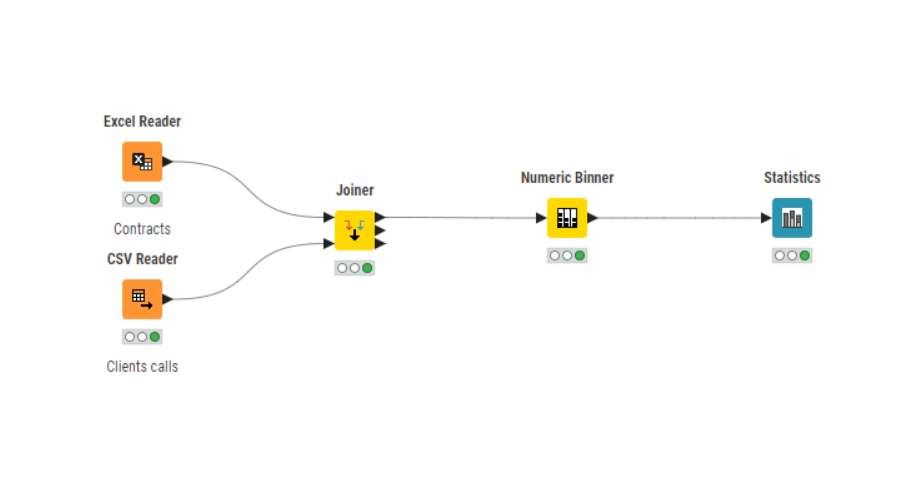
\includegraphics[scale=0.6]{T1/P1-leitura.png}
    \caption{Circuito da tarefa 1}
    \label{fig:enter-label}
\end{figure}

\begin{figure}[h]
    \centering
    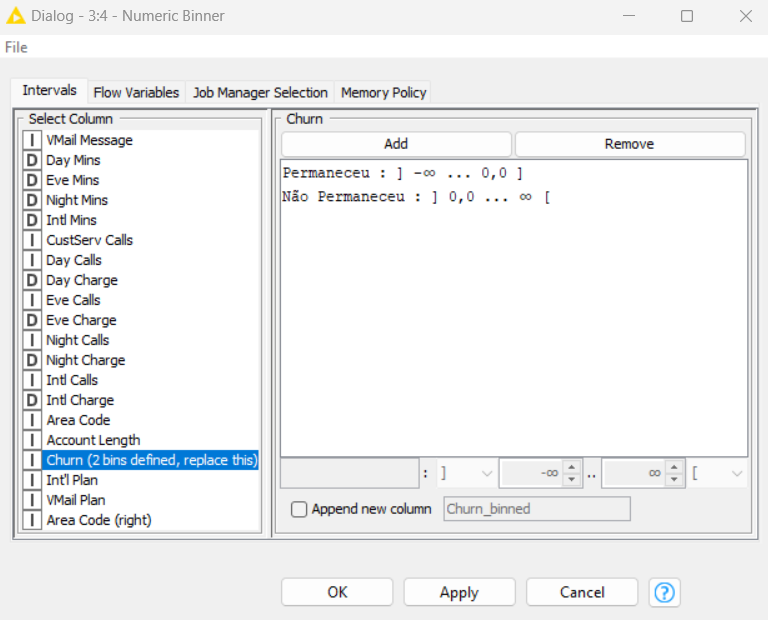
\includegraphics[height=8cm]{T1/P1-Binner.png}
    \caption{Configuração do Numeric Binner}
    \label{fig:enter-label}
\end{figure}

\vspace{10cm}

\begin{figure}[h]
    \centering
    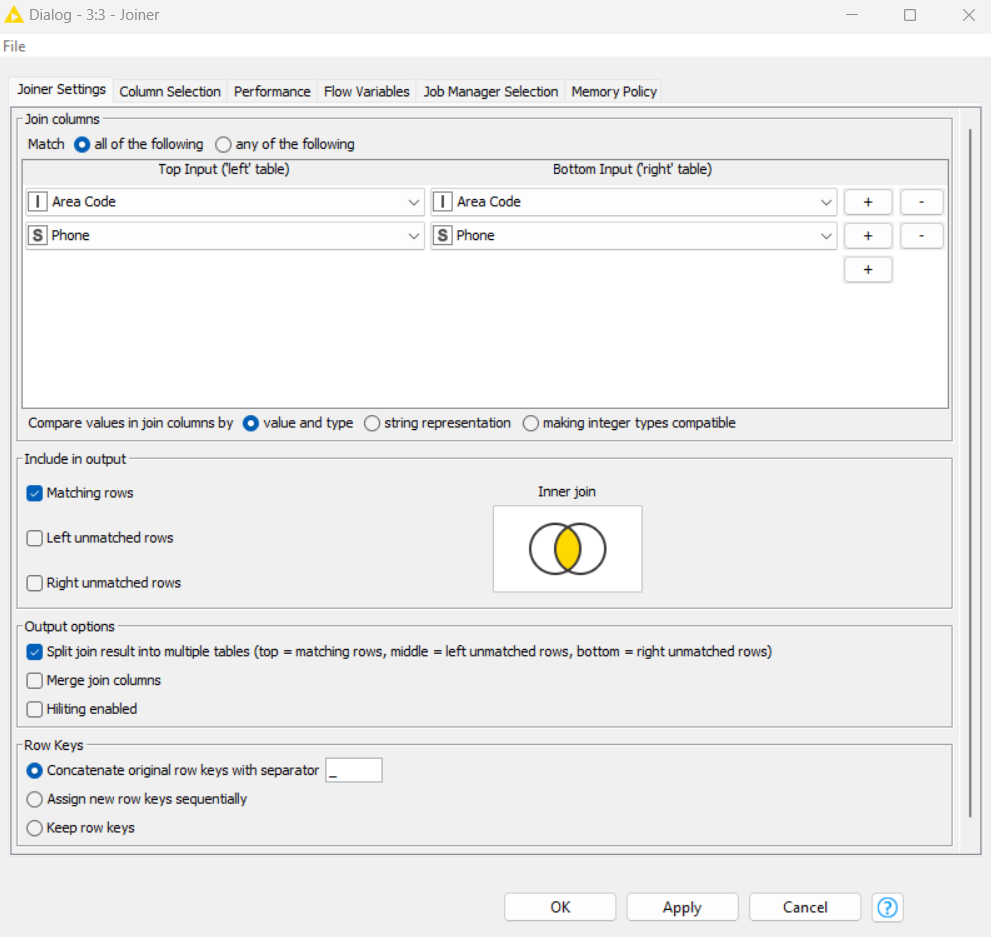
\includegraphics[scale=0.7]{T1/P1-Joiner.png}
    \caption{Configuração do Joiner}
    \label{fig:enter-label}
\end{figure}

Na Figura 1 vemos a configuração do Joiner, onde realizamos a agregação com base nos campos \textit{Area Code} e \textit{Phone}.   


Na Figura 2 temos a configuração do \textit{Numeric Binner}, utilizado para transformar o atributo \textit{Churn} em nominal. 

Por fim, na Figura 3 temos o circuito completo, com a leitura dos respetivos dados.

\newpage

\subsection{Tarefa 2}
\textbf{Enunciado: }Aplicar nodos para exploração de dados, i.e., analisar os dados em relação às suas características e padrões, procurando extrair informação relevante dos dados.  
\newline


\begin{figure}[htp]
    
    \centering
     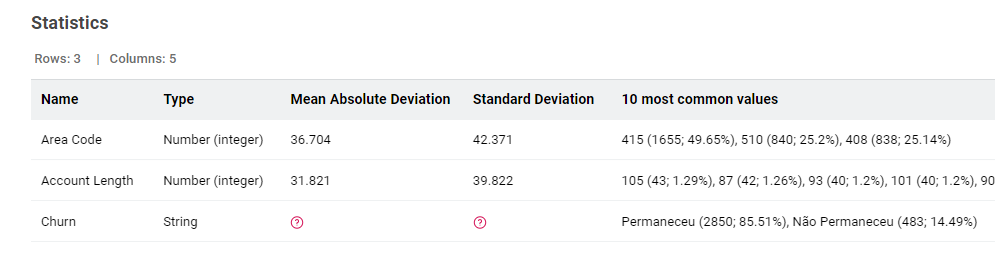
\includegraphics[width=\textwidth]{T2/P2-Stats.png}
     \caption{Estatísticas de Churn}

     \centering
     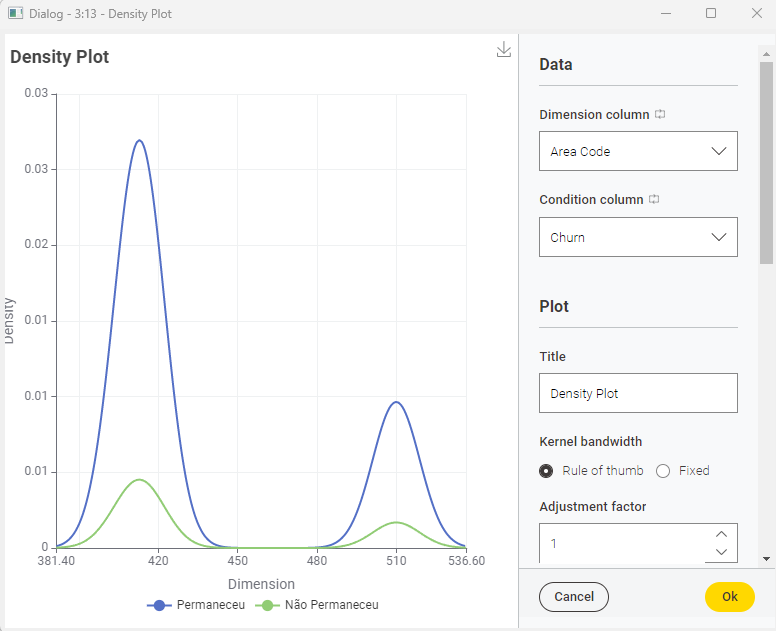
\includegraphics[height=10cm]{T2/P2-DensityChurn.png}
     \caption{Densidade de Churn}

\end{figure}

Nesta tarefa analisei alguns dados resultantes de aplicar os nodos anteriormente demonstrados. Com efeito, na Figura 4 vemos algumas estatísticas de Churn, após remoção de algumas colunas. Repare-se que 85.51\% das pessoas permaneceram na companhia.

Na figura 5 apliquei um nodo de densidade e relacionei a Area Code na \textbf{Dimension Column} com o Churn na \textbf{Condition Column} e observa-se que há maior frequência de clientes a viver nas zonas 380 - 450, comparativamente às zonas 480 - 540 mas a frequência de Churn não varia muito. 

\newpage

\subsection{Tarefa 3}
\textbf{Enunciado:} Particionar os dados de forma estratificada (pela feature “Churn”), utilizando 70\% para aprendizagem e 30\% para teste. Aplicar um Decision Tree Learner e um Decision Tree Predictor. Avaliar a precisão (accuracy) do modelo e a respetiva matriz de confusão;

\begin{figure}[htp]
    
    \centering
     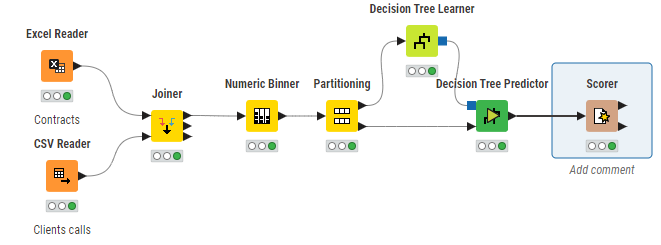
\includegraphics[scale=1]{T3/Circuito.png}
     \caption{Circuito Completo}
    \vspace{0.5cm}
     \centering
     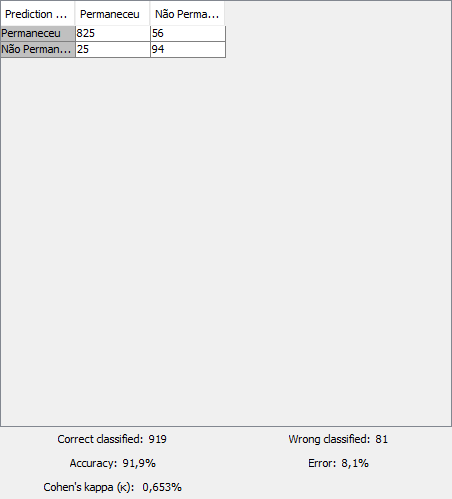
\includegraphics[scale=0.5]{T3/ConfusionMatrix.png}
     \caption{Matriz de Confusão}
\end{figure} 

Nesta tarefa, inicialmente utilizei o nodo \textbf{Partitioning} para realizar a partição pedida, aplicando de seguida a Decision Tree. Como resultado obtemos 919(825+94) casos positivos e 81(25+56) casos negativos, resultando numa accuracy de 91.9\%. 

Consideremos o coeficiente \textbf{Cohen's kappa} com k=0.653\%, o que significa que em 65.3\% dos casos dois observadores distintos concordariam com as decisões tomadas, tendo em conta casos reais e esperados. 

\newpage

\subsection{Tarefa 4}
\textbf{Enunciado:} Remover, iterativamente, features do dataset e reavaliar a performance dos modelos candidatos. Descrever os resultados obtidos;

\begin{figure}[htp]
    
     \centering
     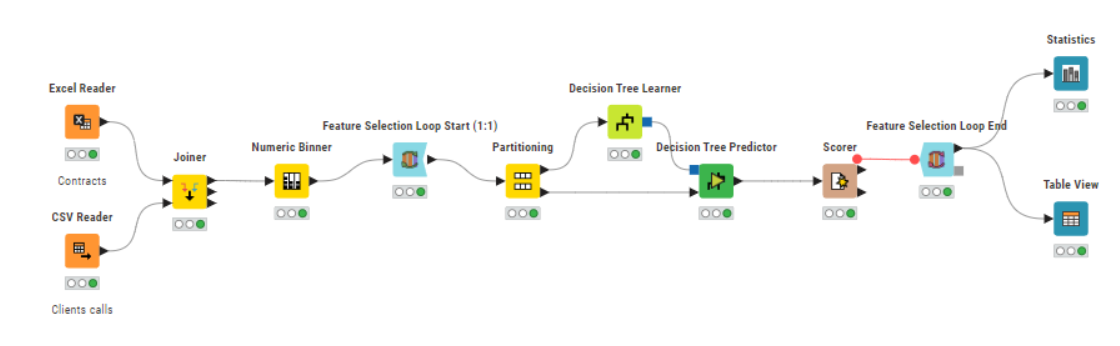
\includegraphics[scale=0.7]{T4/Circuito.png}
     \caption{Circuito Completo}
     \vspace{0.5cm}
     \centering
     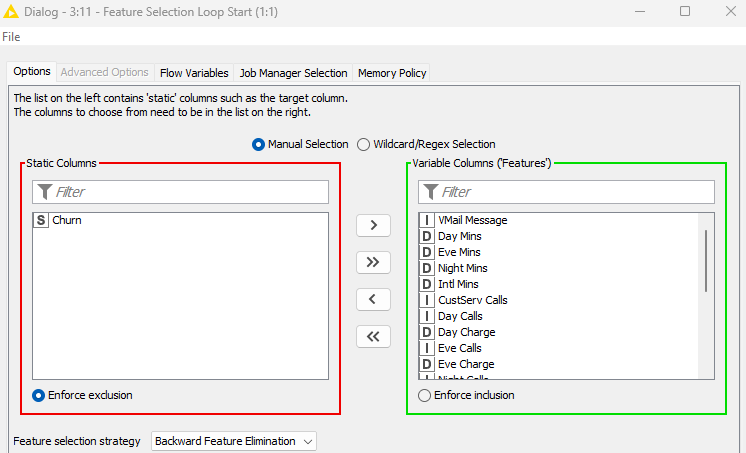
\includegraphics[scale=0.7]{T4/config_loop.png}
     \caption{Configuração do Loop}
\end{figure} 

\begin{figure}
    \centering
    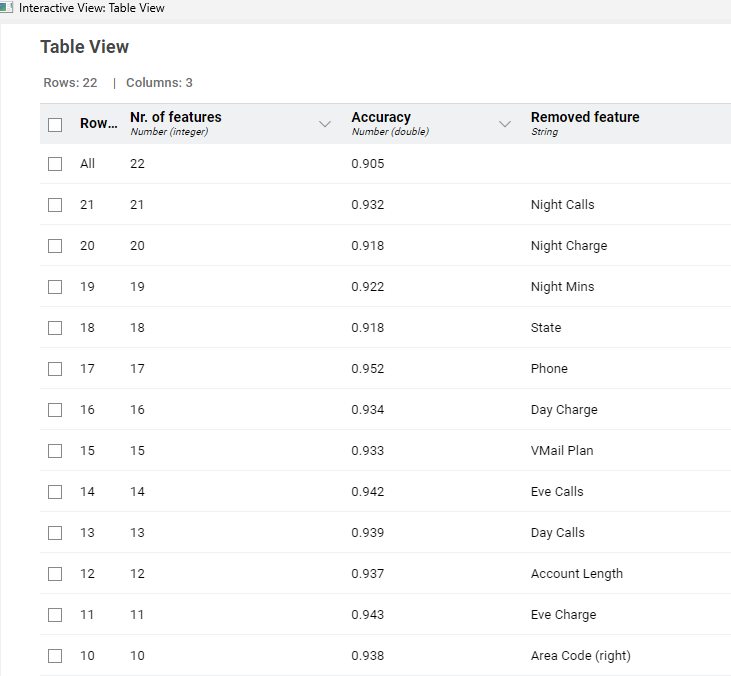
\includegraphics{T4/Stats.png}
    \caption{Table View}
    \label{fig:enter-label}
\end{figure}

\newpage

Inicialmente, na Figura 8 vemos o circuito usado para a resolução do problema, dando especial destaque ao nodo Feature Selection Loop Start, que foi usado para iterativamente remover features do dataset.  

Por sua vez, na Figura 9 é mostrada a configuração do loop, em que o atributo \textit{Churn} foi colocado na coluna static devido ao facto de ser um atributo nominal e em que foi usada a estratégia \textbf{Backward Feature Elimination} para, iterativamente, remover features do dataset.  

Por fim, na Figura 10 vemos a accuracy do modelo com diferentes números de features. Se observarmos a tabela percebemos que até certo ponto a accuracy do nosso modelo aumenta à medida que retiramos features. Isto não é necessariamente boa notícia visto que uma maior quantidade de dados geralmente contribui para um modelo mais sólido. 

Concluo, portanto, que nem sempre a accuracy do modelo é equivalente à qualidade do mesmo.

\newpage

\subsection{Tarefa 5}
\textbf{Enunciado:} Seguir as práticas de bons-hábitos na construção de workflows.

\begin{figure}[htp]
    \centering
    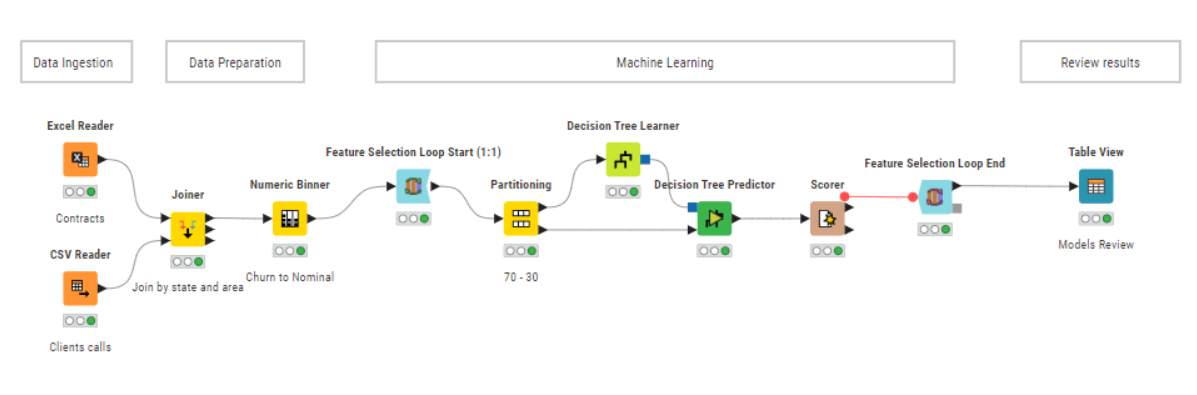
\includegraphics[scale=0.75]{T5/GoodHabits.png}
    \caption{Circuito anotado}
    \label{fig:enter-label}
\end{figure}

Na tarefa 5 procurei seguir boas práticas na construção de workflows através da utilização de notas, que marcam as diferentes fases do meu circuito. Para além disso também nomeei alguns nodos dando a entender de forma simples e sucinta as suas funcionalidades.  

Podia ainda ter utilizado metanodos para compactar o workflow, no entanto, não achei necessário neste caso, visto que o circuito não demonstra grande complexidade.

\newpage

\subsection{Tarefa 6}
\textbf{Enunciado:} Utilizar o output de um nodo Decision Tree Learner para criar uma imagem de uma Árvore de Decisão e guardar essa imagem no ambiente de trabalho.

\begin{figure}[htp]
    \centering
    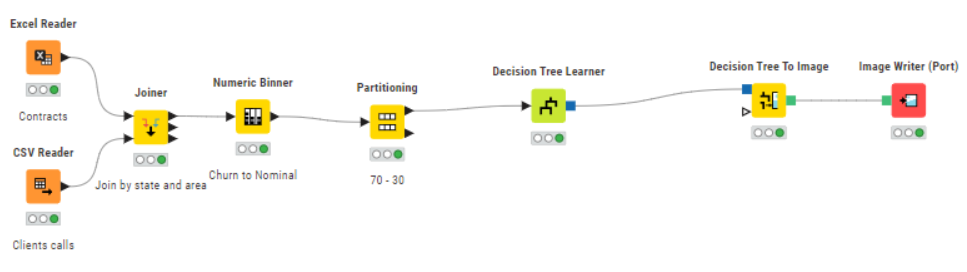
\includegraphics[scale=0.8]{T6/Circuito.png}
    \caption{Workflow usado para representação em imagem}
    \label{fig:enter-label}
    \vspace{1cm}
    \centering
    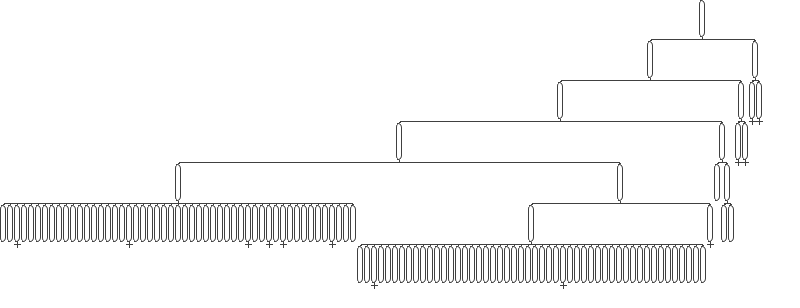
\includegraphics[scale=0.7]{T6/decision_tree.png}
    \caption{Decision Tree em formato PNG}
    \label{fig:enter-label}
    
\end{figure}

Para finalizar, utilizei o nodo \textbf{Decision Tree To Image} para converter o modelo para imagem, e de seguida utilizei o nodo \textbf{Image Writer} para guardar a imagem resultante. O resultado final está expresso na Figura 13.

\newpage

\section{Conclusão}
Para concluir, esta tarefa foi importante, principalmente, para o conhecimento de novos nodos do knime e para desenvolver a minha capacidade na análises de dados.  



\newpage
\end{document}



